\chapter{Modeling}

\begin{figure}[hbtp]
	\centering
	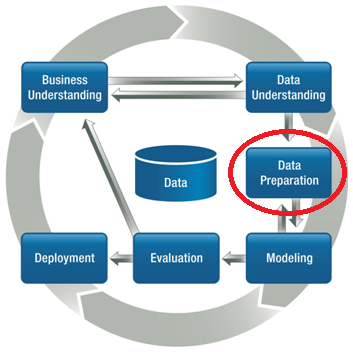
\includegraphics[width=0.5\textwidth]{./images/CRISPDM_3.png}
	\caption{CRISP-DM - Modeling}
	\label{CRISPDM_4}
\end{figure}

\section{Tecnica di Modeling}
Ai fini della classificazione, si è deciso di modellare il dataset realizzando un albero di decisione funzionale. In particolare si è utilizzato l'algoritmo \textbf{FT} (\textit{\textbf{F}unctional \textbf{T}ree}).

\section{Rappresentazione del Modello}

Classifier for building 'Functional trees', which are classification trees  that could have logistic regression functions at the inner nodes and/or leaves. The algorithm can deal with binary and multi-class target variables, numeric and nominal attributes and missing values.\cite{Gama2004}

modelType -- The type of FT model. 0, for FT, 1, for FTLeaves, and 2, for FTInner

\paragraph{Functional Trees}
Dato un set di esempi e un costruttore di attributi, l'algoritmo generale usato per la costruzione dell'albero funzionale è mostrato di seguito. Questo algoritmo è molto simile a molti altri, fatta eccezione nella fase di costruzione (Fasi 2 e 3). Qui viene creata una nuova funzione e mappata ai nuovi attributi creati. Ci sono alcuni aspetti di questo algoritmo che devono essere esplicitati. Nella fase 2, il modello viene costruito usando la funzione costruttore. Questo viene fatto usando solo gli esempi che ricadono in questo nodo. Successivamente, nella fase 3, il modello viene mappato ai nuovi attributi. La funzione costruttore deve essere o un classificatore o un regressore in base alla tipologia di problema. Il numero dei nuovi attributi da creare, sarà uguale al numero delle classi che si hanno a disposizione; Infine, la funzione costruttore \textbf{is mapped to one new attribute}. Nella fase 3, ogni nuovo attributo è computato come valore predetto dalla funzione costruita per ogni esempio. In caso di classificazione, ogni nuovo attributo-valore sarà la probabilità che quell'esempio appartenga ad una delle classi date dal modello costruito.
Il valore di ogni nuovo attributo viene valutato usando la funzione di merito di un albero univariato tenendo conto sempre dei valori originali degli attributi (Fase 4). Il modello costruito dall'algoritmo ha due tipi di nodi decisionali: Quelli basati sul test di uno degli attributi originali, e quelli basati sul valore della funzione costruttore. Quando si usa un modello lineare generalizzato (GLM) come costruttore di attributi, ogni nuovo attributo è una combinazione lineare degli attributi originali. I nodi decisionali basati sugli attributi costruiti, definiscono un piano di decisione multivariato.

\begin{figure}[hbtp]
	\centering
	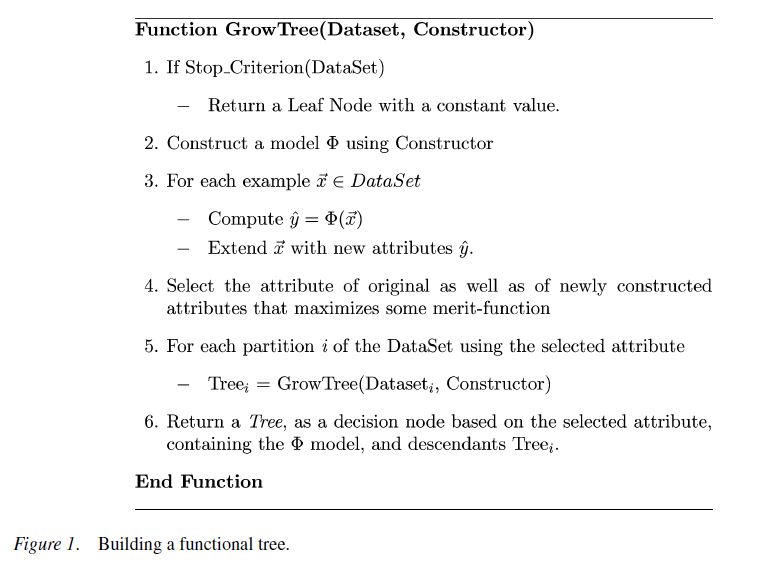
\includegraphics[width=0.9\textwidth]{./images/FunctionGrowTree.JPG}
	\caption{Function GrowTree}
\end{figure}

\textbf{Function GrowTree(Dataset, Constructor)}
\begin{enumerate}
	\item If $Stop\_Criterion(DataSet)$
	\begin{itemize}
		\item Return a Leaf Node with a constant value.
	\end{itemize}
	\item Construct a model $\Phi$ using Constructor
	\item For each example $\vec{x} \in DataSet$
	\begin{itemize}
		\item Compute $\hat y = \Phi(\vec{x})$
		\item Extend $\vec{x}$ with new attributes $\hat y$.
	\end{itemize}
	\item Select the attribute of original as well as of newly constructed attributes that maximizes some merit-function \label{selection}
	\item For each partition $i$ of the DataSet using the selected attribute
	\begin{itemize}
		\item $Tree_{i} = GrowTree (Dataset_{i},Constructor)$
	\end{itemize}
	\item Return a $Tree$, as a decision node based on the selected attribute, contaning the $\Phi$ model, and descendants $Tree_{i}$.
\end{enumerate}
\textbf{End Function}

Una volta creato l'albero, si passa alla fase di potatura. L'algoritmo generale di potatura verrà mostrato in seguito. L'albero viene visitato usando un approccio bottom-up (Post-visita). Per ogni nodo non foglia vengono stimati due valori quantitativi: 
\begin{itemize}
	\item Errore statico;
	\item Errore di "Backed-up"
\end{itemize}
L'\textbf{errore statico} è la stima dell'errore se il nodo fosse foglia.
L'\textbf{errore di backed-up} è la somma pesata della stima degli errori di tutti i sotto alberi del nodo corrente. La stima dell'errore di ogni ramo è pesato usando la probabilità che un esempio appartenga al ramo. Se l'errore di "Backed-up" è più grande o uguale all'errore statico, il nodo verrà sostituito da una foglia avente come valore, il valore dato dalla classe di maggioranza del nodo. L'aspetto fondamentale dell'algoritmo di potatura è l'errore stimato nella fase 1. Ad ogni nodo, sarà necessario stimare la probabilità dell'errore dato l'errore nel campione degli esempi che ricadono in questo nodo. La probabilità dell'errore non può essere determinato esattamente. Per un dato livello di confidenza, otteniamo un intervallo di confidenza [Lcf; Ucf] con una probabilità di 1-cf che contenga l'errore reale.


As in Quinlan (1993a), we use the upper limit of the confidence
interval Ucf as a pessimistic estimation for the true error.
The confidence interval for the error depends on the loss-function used. In classification
problems, and under the 0-1 loss, the error is governed by a Binomial distribution (Mitchell,
1997). In regression problems, and for the squared error loss the variance of the error for
a given example follows a χ2 distribution. For a set of examples the sum of χ2 can be
approximated using a Normal distribution (Bhattacharyya \& Johnson, 1977). For each
node, the upper limit of the confidence interval is obtained from the sample error using
the appropriate distribution. A similar procedure is used to estimate the constructor error
(step 3).
The pruning algorithm produces two different type of leaves: ordinary leaves that predict
a constant, and constructor leaves that predict the value of the constructor function learned
(in the growing phase) at this node.
We obtain different conceptual models by simplifying our algorithm. Two interesting
simplifications are described in the following sub-sections.

%Given a set of examples and an attribute constructor, the general algorithm used to build a
%functional tree is presented in figure 1. This algorithm is similar to many others, except in the constructive phase (steps 2 and 3). Here a function is built and mapped to new attributes.
%There are some aspects of this algorithm that should be made explicit. In step 2, a model
%is built using the constructor function. This is done using only the examples that fall at
%this node. Later, in step 3, the model is mapped to new attributes. The constructor function
%should be a classifier or a regressor depending on the type of the problem. In the former
%the number of new attributes is equal to the number of classes(At different nodes the system considers different number of classes depending on the class distribution of the
%examples that fall at this node.), in the latter the constructor
%function is mapped to one new attribute. In step 3, each new attribute is computed as the
%value predicted by the constructed function for each example. In the classification setting,
%each new attribute-value is the probability that the example belongs to one class given by
%the constructed model.
%The merit of each new attribute is evaluated using the merit-function of the univariate tree,
%and in competition with the original attributes (step 4). The model built by our algorithm
%has two types of decision nodes: those based on a test of one of the original attributes,
%and those based on the values of the constructor function. When using generalized linear
%models (GLM) as the attribute constructor, each new attribute is a linear combination of
%the original attributes. Decision nodes based on constructed attributes define a multivariate
%decision surface. 
%%Once a tree has been built, it is pruned back. The general algorithm to prune the tree is presented in figure 2. The tree is traversed using a bottom-up, post-order strategy. For each non-leaf node two quantities are estimated: the static error and the backed-up error. Static error is an estimation of the error as if the node were a leaf. Backed-up error is the weighted sum of the estimation of the errors of all subtrees of the current node. The estimation of the error of each branch is weighted by the probability that an example follows the branch. If backed-up error is greater or equal than static error, then the node is replaced by a leaf with the majority class of the node.
%The fundamental aspect of the pruning algorithm is the error estimation in step 1. At each
%node, we need to estimate the probability of error given the error in the sample of examples
%that fall at this node. The probability of error cannot be determined exactly. For a given
%confidence level we can obtain a confidence interval [Lcf ;Ucf ] that with probability 1−cf contains the true error. 

% \begin{figure}[hbtp]
% 	\centering
% 	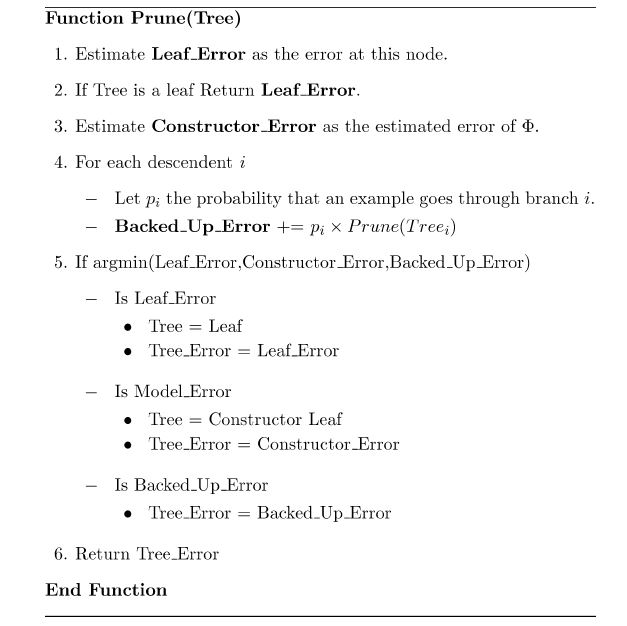
\includegraphics[width=0.5\textwidth]{./images/FunctionGrowTreePrune.JPG}
% 	\caption{Function GrowTree Prune}
% \end{figure}

\textbf{Function Prune (Tree)}
 \begin{enumerate}
 	\item Estimate \textbf{Leaf\_Error} as the error at this node.
	\item If Tree is leaf Return \textbf{Leaf\_Error}.
 	\item Estimate \textbf{Constructor\_Error} as the estimated error of $\Phi$.
 	\item For each descendent $i$
 	\begin{itemize}
 		\item Let $p_i$ the probability that an example goes through branch $i$.
 		\item \textbf{Backed\_Up\_Error} $+= p_i \times Prune \left(Tree_i\right)$
 	\end{itemize}
 	\item If argmin (Leaf\_Error, Constructor\_Error, Backed\_up\_error)
 	\begin{itemize}
 		\item Is Leaf\_Error
 		\begin{itemize}
 			\item Tree = Leaf
			\item Tree\_Error = Leaf\_Error
 		\end{itemize}
 		\item Is Model Error
 		\begin{itemize}
 			\item Tree = Constructor Leaf
 			\item Tree\_Error = Constructor\_Error
 		\end{itemize}
 		\item Is Backed\_Up\_Error
 		\begin{itemize}
 			\item Tree\_Error = Backed\_Up\_Error
 		\end{itemize}
 	\end{itemize}	
 \end{enumerate} 
\textbf{End Function}

\paragraph{Functional leaves only}
Utilizzando l'approccio FT-Leaves, il modello funzionale non viene utilizzato nei test per effettuare lo splitting, ma solo ed esclusivamente nelle foglie. In questo approccio, si restringe la selezione degli attributi di test, ai soli attributi originali. (Fase \ref{selection} nell'algoritmo di crescita)
Questo è l'approccio utilizzato ad esempio nell'M5 di Quinlan \cite{Quinlan93combininginstance-based}, e nel sistema NBtree \cite{Kohavi1996}. 
Tuttavia, ad ogni nodo viene costruita la funzione costruttore che verrà poi utilizzata nella fase di pruning dell'albero. In questo modo, tutti i nodi decisionali sono basati sugli attributi di partenza. I nodi foglia potrebbero contenere il modello costruttore. Un nodo foglia conterrà il modello costruttore se e solo se nell'algoritmo di pruning l'errore stimato del modello costruttore è inferiore sia al "backed-up-error" che allo "static error". Un albero funzionale FT-Leaves divide lo spazio di input in Iper-rettagoli. I dati in ogni regione vengono adattati usando la funzione costruttore.
%Nevertheless we still build, at each node, the constructor function. The model built by the constructor function is used later in the pruning phase. In this way, all decision nodes are based on the original attributes. Leaf nodes could contain a constructor model. A leaf node contains a constructor model if and only if in the pruning algorithm the estimated error of the constructor model is lower than both the Backed-up-error and the Static error. A FT-Leaves functional tree divides the input space into hyper-rectangles. The data in each region could be fitted with the constructor function.

\paragraph{Functional inner nodes only}
Utilizzando l'approccio FT-Inner, si otterranno degli alberi funzionali nel quale i modelli multivariati verranno usati esclusivamente ai nodi decisionali (nodi interni) e non verranno mai usati come classificatori nei nodi foglia. In questo caso, l'algoritmo di pruning verrà limitato alla sola scelta tra il "Backed-up-Error" e lo "Static Error", facendo in modo che, nelle foglie, siano presenti solo i valori costanti utili alla classificazione diretta. Questo approccio è utilizzato in sistemi come LMDT (Utgoff \& Brodley, 1991), OC1 (Murthy, Kasif, \& Salzberg, 1994), LTREE (Gama, 1997), and QUEST (Loh \& Shih, 1997). Un albero funzionale FT-Inner divide lo spazio di input in superfici decisionali oblique. I dati in ogni regione vengono adattati usando la costante che minimizza la funzione di perdita data.
%\paragraph{Functional inner nodes only} We denote as FT-Inner the approach to functional trees where the multivariate models are used exclusively at decision nodes (internal nodes) and not used as classifiers in leaves. In our algorithm, restricting the pruning algorithm to choose only between the Backed-up-Error and the Static error generates this kind of model. In this case all leaves predict a constant value. This is the strategy used in systems like LMDT (Utgoff & Brodley, 1991), OC1 (Murthy, Kasif, & Salzberg, 1994), LTREE (Gama, 1997), and QUEST (Loh & Shih, 1997). A FT-Inner functional tree divides the input space into oblique decision surfaces. The data in each region is fitted with a constant that minimizes the given loss function.

%\paragraph{Prediction using functional trees}
%Once a functional tree has been built, it can be
%used to predict the value of the target attribute for unclassified examples. As usual, the
%example traverses the tree from the root node to a leaf. At each decision node (inner node)
%of the tree the set of attributes of the example is extended using the constructor function
%built at this node. After this expansion, the decision test of the node is applied defining the
%path that the example will follow. When a leaf is reached the example is classified using
%either the constant associated with the leaf or the constructor function built at this leaf.

\section{Valutazione del Modello}

\section{Ricerca}

\section{Test Design}

\section{Costruzione del Modello}

Esempio di costruzione del modello sul training set epurato da attributi in seguito all'esecuzione dell'algoritmo \textit{CfsSubsetEval} definito nel paragrafo \ref{Feature Selection}.
%
%=== Classifier model (full training set) ===
%
%FT tree 
%------------------
%
%N0#1 <= 0.536896
%|   id <= 372407
%|   |   N0#3 <= 0.13727: FT_1:15/60 (4879)
%|   |   N0#3 > 0.13727
%|   |   |   N0#5 <= 0.67676
%|   |   |   |   N0#6 <= 0.363825: Class=1
%|   |   |   |   N0#6 > 0.363825: Class=0
%|   |   |   N0#5 > 0.67676: Class=0
%|   id > 372407: Class=0
%N0#1 > 0.536896
%|   N0#11 <= 0.966266
%|   |   N0#12 <= 0.694099: Class=1
%|   |   N0#12 > 0.694099: Class=0
%|   N0#11 > 0.966266: Class=0
%
%Number of Leaves  : 	8
%
%Size of the Tree : 	15
%FT_N0#1:
%Class 0 :
%-1.33 + 
%[id] * 0    +
%[BASE64_ENC_TEXT] * 1.89 +
%[CLICK_BELOW] * 0.82 +
%[CTYPE_JUST_HTML] * 2.06 +
%[FROM_ENDS_IN_NUMS] * 0.71 +
%[INVALID_DATE] * 1.07 +
%[MISSING_MIMEOLE] * 1.86 +
%[RESENT_TO] * 1.04 +
%[SPAM_PHRASE_00_01] * -1.42 +
%[USER_AGENT_PINE] * -0.69 +
%[WEB_BUGS] * 0.9  +
%[X_ACCEPT_LANG] * -0.68
%
%Class 1 :
%1.33 + 
%[id] * 0    +
%[BASE64_ENC_TEXT] * -1.89 +
%[CLICK_BELOW] * -0.82 +
%[CTYPE_JUST_HTML] * -2.06 +
%[FROM_ENDS_IN_NUMS] * -0.71 +
%[INVALID_DATE] * -1.07 +
%[MISSING_MIMEOLE] * -1.86 +
%[RESENT_TO] * -1.04 +
%[SPAM_PHRASE_00_01] * 1.42 +
%[USER_AGENT_PINE] * 0.69 +
%[WEB_BUGS] * -0.9 +
%[X_ACCEPT_LANG] * 0.68
%
%
%FT_N0#3:
%Class 0 :
%-1.24 + 
%[APPROVED_BY] * -0.53 +
%[BAD_CREDIT] * 1.5  +
%[BASE64_ENC_TEXT] * 2.93 +
%[BIG_FONT] * 0.68 +
%[CLICK_BELOW] * 0.82 +
%[CTYPE_JUST_HTML] * 2.06 +
%[DATE_IN_FUTURE_06_12] * 1.47 +
%[DIET] * 2.56 +
%[FORGED_HOTMAIL_RCVD] * 1.21 +
%[FROM_ENDS_IN_NUMS] * 0.71 +
%[INVALID_DATE] * 1.07 +
%[MIME_HTML_NO_CHARSET] * 1.43 +
%[MISSING_MIMEOLE] * 1.86 +
%[NORMAL_HTTP_TO_IP] * 2.18 +
%[ONLY_COST] * 2.69 +
%[PLING_QUERY] * 0.95 +
%[QUOTED_EMAIL_TEXT] * -1.08 +
%[REMOVE_PAGE] * 1.89 +
%[RESENT_TO] * 1.99 +
%[SPAM_PHRASE_00_01] * -0.8 +
%[SUBJECT_MONTH] * -0.44 +
%[TRACKER_ID] * 2.16 +
%[USER_AGENT_PINE] * -1.82 +
%[WEB_BUGS] * 0.2  +
%[X_ACCEPT_LANG] * -1.14
%
%Class 1 :
%1.24 + 
%[APPROVED_BY] * 0.53 +
%[BAD_CREDIT] * -1.5 +
%[BASE64_ENC_TEXT] * -2.93 +
%[BIG_FONT] * -0.68 +
%[CLICK_BELOW] * -0.82 +
%[CTYPE_JUST_HTML] * -2.06 +
%[DATE_IN_FUTURE_06_12] * -1.47 +
%[DIET] * -2.56 +
%[FORGED_HOTMAIL_RCVD] * -1.21 +
%[FROM_ENDS_IN_NUMS] * -0.71 +
%[INVALID_DATE] * -1.07 +
%[MIME_HTML_NO_CHARSET] * -1.43 +
%[MISSING_MIMEOLE] * -1.86 +
%[NORMAL_HTTP_TO_IP] * -2.18 +
%[ONLY_COST] * -2.69 +
%[PLING_QUERY] * -0.95 +
%[QUOTED_EMAIL_TEXT] * 1.08 +
%[REMOVE_PAGE] * -1.89 +
%[RESENT_TO] * -1.99 +
%[SPAM_PHRASE_00_01] * 0.8  +
%[SUBJECT_MONTH] * 0.44 +
%[TRACKER_ID] * -2.16 +
%[USER_AGENT_PINE] * 1.82 +
%[WEB_BUGS] * -0.2 +
%[X_ACCEPT_LANG] * 1.14
%
%FT_1:
%Class 0 :
%-1.35 + 
%[APPROVED_BY] * -1.04 +
%[BAD_CREDIT] * 1.5  +
%[BASE64_ENC_TEXT] * 2.93 +
%[BIG_FONT] * 0.14 +
%[BUGZILLA_BUG] * -0.51 +
%[CLICK_BELOW] * 3.5  +
%[CRON_ENV] * -0.52 +
%[CTYPE_JUST_HTML] * 2.06 +
%[DATE_IN_FUTURE_06_12] * 1.47 +
%[DIET] * 2.56 +
%[FORGED_HOTMAIL_RCVD] * 1.21 +
%[FROM_ENDS_IN_NUMS] * 0.71 +
%[INVALID_DATE] * 1.07 +
%[MIME_HTML_NO_CHARSET] * 1.43 +
%[MISSING_MIMEOLE] * 1.86 +
%[NORMAL_HTTP_TO_IP] * 2.18 +
%[ONLY_COST] * 2.69 +
%[PLING_QUERY] * 1.7  +
%[QUOTED_EMAIL_TEXT] * -1.59 +
%[REMOVE_PAGE] * 1.89 +
%[RESENT_TO] * 1.99 +
%[SIGNATURE_LONG_SPARSE] * -0.51 +
%[SPAM_PHRASE_00_01] * -0.65 +
%[SUBJECT_MONTH] * -1.46 +
%[SUBJ_MISSING] * -0.52 +
%[TRACKER_ID] * 2.16 +
%[USER_AGENT_PINE] * -2.37 +
%[WEB_BUGS] * 0.2  +
%[X_ACCEPT_LANG] * -1.57
%
%Class 1 :
%1.35 + 
%[APPROVED_BY] * 1.04 +
%[BAD_CREDIT] * -1.5 +
%[BASE64_ENC_TEXT] * -2.93 +
%[BIG_FONT] * -0.14 +
%[BUGZILLA_BUG] * 0.51 +
%[CLICK_BELOW] * -3.5 +
%[CRON_ENV] * 0.52 +
%[CTYPE_JUST_HTML] * -2.06 +
%[DATE_IN_FUTURE_06_12] * -1.47 +
%[DIET] * -2.56 +
%[FORGED_HOTMAIL_RCVD] * -1.21 +
%[FROM_ENDS_IN_NUMS] * -0.71 +
%[INVALID_DATE] * -1.07 +
%[MIME_HTML_NO_CHARSET] * -1.43 +
%[MISSING_MIMEOLE] * -1.86 +
%[NORMAL_HTTP_TO_IP] * -2.18 +
%[ONLY_COST] * -2.69 +
%[PLING_QUERY] * -1.7 +
%[QUOTED_EMAIL_TEXT] * 1.59 +
%[REMOVE_PAGE] * -1.89 +
%[RESENT_TO] * -1.99 +
%[SIGNATURE_LONG_SPARSE] * 0.51 +
%[SPAM_PHRASE_00_01] * 0.65 +
%[SUBJECT_MONTH] * 1.46 +
%[SUBJ_MISSING] * 0.52 +
%[TRACKER_ID] * -2.16 +
%[USER_AGENT_PINE] * 2.37 +
%[WEB_BUGS] * -0.2 +
%[X_ACCEPT_LANG] * 1.57
%
%FT_N0#5:
%Class 0 :
%0.64 + 
%[id] * 0    +
%[APPROVED_BY] * -0.53 +
%[BAD_CREDIT] * 3.02 +
%[BASE64_ENC_TEXT] * 2.93 +
%[BIG_FONT] * 0.33 +
%[CLICK_BELOW] * 0.82 +
%[CTYPE_JUST_HTML] * 2.06 +
%[DATE_IN_FUTURE_06_12] * 1.47 +
%[DIET] * 3.19 +
%[FORGED_HOTMAIL_RCVD] * 1.21 +
%[FROM_ENDS_IN_NUMS] * 0.35 +
%[INVALID_DATE] * 1.7  +
%[MAY_BE_FORGED] * -0.95 +
%[MIME_HTML_NO_CHARSET] * 0.88 +
%[MISSING_MIMEOLE] * 1.86 +
%[NORMAL_HTTP_TO_IP] * 2.64 +
%[ONLY_COST] * 2.69 +
%[PLING_QUERY] * 0.95 +
%[QUOTED_EMAIL_TEXT] * -2.38 +
%[REMOVE_PAGE] * 1.89 +
%[RESENT_TO] * 1.69 +
%[SPAM_PHRASE_00_01] * -0.8 +
%[SUBJECT_MONTH] * 0.47 +
%[TRACKER_ID] * 2.16 +
%[USER_AGENT_PINE] * -1.82 +
%[WEB_BUGS] * 0.2  +
%[X_ACCEPT_LANG] * -3.16
%
%Class 1 :
%-0.64 + 
%[id] * 0    +
%[APPROVED_BY] * 0.53 +
%[BAD_CREDIT] * -3.02 +
%[BASE64_ENC_TEXT] * -2.93 +
%[BIG_FONT] * -0.33 +
%[CLICK_BELOW] * -0.82 +
%[CTYPE_JUST_HTML] * -2.06 +
%[DATE_IN_FUTURE_06_12] * -1.47 +
%[DIET] * -3.19 +
%[FORGED_HOTMAIL_RCVD] * -1.21 +
%[FROM_ENDS_IN_NUMS] * -0.35 +
%[INVALID_DATE] * -1.7 +
%[MAY_BE_FORGED] * 0.95 +
%[MIME_HTML_NO_CHARSET] * -0.88 +
%[MISSING_MIMEOLE] * -1.86 +
%[NORMAL_HTTP_TO_IP] * -2.64 +
%[ONLY_COST] * -2.69 +
%[PLING_QUERY] * -0.95 +
%[QUOTED_EMAIL_TEXT] * 2.38 +
%[REMOVE_PAGE] * -1.89 +
%[RESENT_TO] * -1.69 +
%[SPAM_PHRASE_00_01] * 0.8  +
%[SUBJECT_MONTH] * -0.47 +
%[TRACKER_ID] * -2.16 +
%[USER_AGENT_PINE] * 1.82 +
%[WEB_BUGS] * -0.2 +
%[X_ACCEPT_LANG] * 3.16
%
%FT_N0#6:
%Class 0 :
%1.2  + 
%[id] * 0    +
%[APPROVED_BY] * -0.53 +
%[BAD_CREDIT] * 3.02 +
%[BASE64_ENC_TEXT] * 2.93 +
%[BIG_FONT] * 0.02 +
%[CLICK_BELOW] * 0.82 +
%[CTYPE_JUST_HTML] * 2.06 +
%[DATE_IN_FUTURE_06_12] * -0.46 +
%[DIET] * 3.19 +
%[FORGED_HOTMAIL_RCVD] * 1.21 +
%[FROM_ENDS_IN_NUMS] * 0.35 +
%[INVALID_DATE] * 1.7  +
%[MAY_BE_FORGED] * -0.66 +
%[MIME_HTML_NO_CHARSET] * -0.29 +
%[MISSING_MIMEOLE] * 1.86 +
%[NORMAL_HTTP_TO_IP] * 1.56 +
%[ONLY_COST] * 2.69 +
%[PLING_QUERY] * 0.95 +
%[QUOTED_EMAIL_TEXT] * -2.38 +
%[REMOVE_PAGE] * -0.19 +
%[RESENT_TO] * 1.69 +
%[SPAM_PHRASE_00_01] * -0.8 +
%[SUBJECT_MONTH] * 0.47 +
%[TRACKER_ID] * 0.54 +
%[USER_AGENT_PINE] * -1.82 +
%[WEB_BUGS] * 0.2  +
%[X_ACCEPT_LANG] * -3.16
%
%Class 1 :
%-1.2 + 
%[id] * 0    +
%[APPROVED_BY] * 0.53 +
%[BAD_CREDIT] * -3.02 +
%[BASE64_ENC_TEXT] * -2.93 +
%[BIG_FONT] * -0.02 +
%[CLICK_BELOW] * -0.82 +
%[CTYPE_JUST_HTML] * -2.06 +
%[DATE_IN_FUTURE_06_12] * 0.46 +
%[DIET] * -3.19 +
%[FORGED_HOTMAIL_RCVD] * -1.21 +
%[FROM_ENDS_IN_NUMS] * -0.35 +
%[INVALID_DATE] * -1.7 +
%[MAY_BE_FORGED] * 0.66 +
%[MIME_HTML_NO_CHARSET] * 0.29 +
%[MISSING_MIMEOLE] * -1.86 +
%[NORMAL_HTTP_TO_IP] * -1.56 +
%[ONLY_COST] * -2.69 +
%[PLING_QUERY] * -0.95 +
%[QUOTED_EMAIL_TEXT] * 2.38 +
%[REMOVE_PAGE] * 0.19 +
%[RESENT_TO] * -1.69 +
%[SPAM_PHRASE_00_01] * 0.8  +
%[SUBJECT_MONTH] * -0.47 +
%[TRACKER_ID] * -0.54 +
%[USER_AGENT_PINE] * 1.82 +
%[WEB_BUGS] * -0.2 +
%[X_ACCEPT_LANG] * 3.16
%
%
%
%
%
%FT_N0#11:
%Class 0 :
%-0.45 + 
%[id] * 0    +
%[BASE64_ENC_TEXT] * 1.89 +
%[CLICK_BELOW] * 0.82 +
%[CTYPE_JUST_HTML] * 2.44 +
%[FORGED_HOTMAIL_RCVD] * 0.55 +
%[FROM_ENDS_IN_NUMS] * -0.38 +
%[INVALID_DATE] * 1.07 +
%[MAY_BE_FORGED] * 0.57 +
%[MIME_HTML_NO_CHARSET] * 0.56 +
%[MISSING_MIMEOLE] * 1.86 +
%[ONLINE_PHARMACY] * 0.69 +
%[ONLY_COST] * 0.57 +
%[PLING_QUERY] * 1.12 +
%[QUOTED_EMAIL_TEXT] * -1.32 +
%[RESENT_TO] * 1.36 +
%[SPAM_PHRASE_00_01] * -1.42 +
%[TRACKER_ID] * 0.63 +
%[USER_AGENT_PINE] * -0.69 +
%[WEB_BUGS] * 1.36 +
%[X_ACCEPT_LANG] * -0.68
%
%Class 1 :
%0.45 + 
%[id] * 0    +
%[BASE64_ENC_TEXT] * -1.89 +
%[CLICK_BELOW] * -0.82 +
%[CTYPE_JUST_HTML] * -2.44 +
%[FORGED_HOTMAIL_RCVD] * -0.55 +
%[FROM_ENDS_IN_NUMS] * 0.38 +
%[INVALID_DATE] * -1.07 +
%[MAY_BE_FORGED] * -0.57 +
%[MIME_HTML_NO_CHARSET] * -0.56 +
%[MISSING_MIMEOLE] * -1.86 +
%[ONLINE_PHARMACY] * -0.69 +
%[ONLY_COST] * -0.57 +
%[PLING_QUERY] * -1.12 +
%[QUOTED_EMAIL_TEXT] * 1.32 +
%[RESENT_TO] * -1.36 +
%[SPAM_PHRASE_00_01] * 1.42 +
%[TRACKER_ID] * -0.63 +
%[USER_AGENT_PINE] * 0.69 +
%[WEB_BUGS] * -1.36 +
%[X_ACCEPT_LANG] * 0.68
%
%FT_N0#12:
%Class 0 :
%-0.68 + 
%[id] * 0    +
%[BASE64_ENC_TEXT] * 1.89 +
%[BIG_FONT] * -0.36 +
%[CLICK_BELOW] * 0.82 +
%[CTYPE_JUST_HTML] * 2.44 +
%[DIET] * 1.27 +
%[FORGED_HOTMAIL_RCVD] * 0.55 +
%[FROM_ENDS_IN_NUMS] * -0.38 +
%[HTML_COMMENT_SAVED_URL] * 0.58 +
%[INVALID_DATE] * 1.07 +
%[MAILTO_TO_REMOVE] * 1.13 +
%[MAY_BE_FORGED] * 0.57 +
%[MIME_HTML_NO_CHARSET] * 0.56 +
%[MISSING_MIMEOLE] * 1.67 +
%[ONLINE_PHARMACY] * 1.32 +
%[ONLY_COST] * 1.26 +
%[PENIS_ENLARGE2] * 1.26 +
%[PLING_QUERY] * 1.12 +
%[QUOTED_EMAIL_TEXT] * -1.32 +
%[RESENT_TO] * 1.78 +
%[SPAM_PHRASE_00_01] * -1.42 +
%[TRACKER_ID] * 1.37 +
%[USER_AGENT_PINE] * -0.69 +
%[WEB_BUGS] * 2.44 +
%[X_ACCEPT_LANG] * -0.68
%
%Class 1 :
%0.68 + 
%[id] * 0    +
%[BASE64_ENC_TEXT] * -1.89 +
%[BIG_FONT] * 0.36 +
%[CLICK_BELOW] * -0.82 +
%[CTYPE_JUST_HTML] * -2.44 +
%[DIET] * -1.27 +
%[FORGED_HOTMAIL_RCVD] * -0.55 +
%[FROM_ENDS_IN_NUMS] * 0.38 +
%[HTML_COMMENT_SAVED_URL] * -0.58 +
%[INVALID_DATE] * -1.07 +
%[MAILTO_TO_REMOVE] * -1.13 +
%[MAY_BE_FORGED] * -0.57 +
%[MIME_HTML_NO_CHARSET] * -0.56 +
%[MISSING_MIMEOLE] * -1.67 +
%[ONLINE_PHARMACY] * -1.32 +
%[ONLY_COST] * -1.26 +
%[PENIS_ENLARGE2] * -1.26 +
%[PLING_QUERY] * -1.12 +
%[QUOTED_EMAIL_TEXT] * 1.32 +
%[RESENT_TO] * -1.78 +
%[SPAM_PHRASE_00_01] * 1.42 +
%[TRACKER_ID] * -1.37 +
%[USER_AGENT_PINE] * 0.69 +
%[WEB_BUGS] * -2.44 +
%[X_ACCEPT_LANG] * 0.68
